\documentclass[a4paper]{report}
\usepackage[T1]{fontenc}
\usepackage[sfdefault]{biolinum}
\usepackage[french]{babel}
\usepackage{setspace}
\usepackage{tabularx}
\usepackage{graphicx}
\usepackage{wrapfig}
\usepackage{float}
\usepackage[headheight=13pt,top=3cm, bottom=2cm, left=1cm, right=1cm]{geometry}
\usepackage{fancyhdr}
\pagestyle{fancy}
\usepackage{hyperref}
\hypersetup{
    colorlinks=true,
    linkcolor=black,
    citecolor=black,
    filecolor=black,
    urlcolor=black,
}
\renewcommand{\headrulewidth}{1pt}
\renewcommand{\footrulewidth}{1pt}
\fancyfoot[L]{ENSIAS}
\fancyfoot[C]{\textbf{\thepage}}
\fancyfoot[R]{Année universitaire: 2020/2021}
\begin{document}
\begin{titlepage}
	\begin{center}
		\begin{figure}[!h]
			\vspace{- 2 cm}
			\hspace{ 0 cm}
			
\includegraphics[width=9em]{images/ensias.jpeg}
		\end{figure}
		\begin{figure}[!h]
			\vspace{- 3.34cm}
			\hspace{15cm}
			
\includegraphics[width=10em]{images/um5.jpeg}
		\end{figure}
	\end{center}

	\begin{center}
		\begin{center}
			\noindent \hspace{ 0.4 cm}{\LARGE \textsc{Rapport de Stage de Fin de deuxième Année}}\\
		\end{center}
		\begin{center}
			\rule{0.9\linewidth}{1pt}
		\end{center}
		\vspace*{0.2cm}
		\noindent \hspace{ 0.3 cm }\Huge \textbf{Création d'une
			plateforme Web pour la gestion et le suivi des contrats du transport
			délégués}
		\begin{center}
			\rule{0.9\linewidth}{1pt}
		\end{center}

		\vspace*{0.5cm} \noindent \hspace{ -0.5 cm} \large
		\begin{figure}[H]
			\begin{center}
				
\includegraphics[scale=0.8]{images/logo-uir2.jpg}
			\end{center}
		\end{figure}
		\textbf{\emph{Préparé par: KOTBI Abderrahamane}}
		\raggedright{\rule{0.7\linewidth}{2pt}}\\
		\textbf{\emph{
				Membres de Jury:\\
				\begin{itemize}
					\item[•] ****
					\item[•] ****
				\end{itemize}
			}}
		\mbox{}\vfill
		\begin{center}
			\rule{0.9\linewidth}{1pt}\\
			\Large\emph{
				Filière Génie Logiciel\\
				Année universitaire: 2020/2021
			}
		\end{center}


	\end{center}
\end{titlepage}

\newpage

\pagenumbering{roman} \setcounter{page}{1}
\begin{doublespace}
	\chapter*{\centering Remerciements}
	\addcontentsline{toc}{chapter}{Remerciements}
	\textit{
		Avant d'aborder la description des parties importantes du projet,
		j'aimerai tout d’abord exprimer ma gratitude
		intense à toute personne qui a contribué énormément dans l'élaboration
		et la réalisation de ce travail. Je commence
		ainsi par offrir mes remerciements à l'intégralité des personnes
		travaillant au sein de l’école Nationale supérieure d’informatique et d’analyse
		des systèmes. Ces bonnes hommes et femmes qui ne cessent de nous préparer, moi
		et
		mes collègues, pour de telles expériences afin de bien s’intégrer dans
		le cadre réelle du marché de travail.
		Toute ma gratitude et profonde reconnaissance s’adressent à à tous mes
		encadrants de stages: Mme.\textbf{***f***} ****,
		M..\textbf{***m***} ****   . Je vous remercie énormément pour m'avoir
		garanti un encadrement de qualité pour bien mener
		et assurer la réalisation de ce travail dans les meilleures des
		conditions.
	}

	\newpage

	\chapter*{\centering Résumé}
	\addcontentsline{toc}{chapter}{Résumé}

	Ce document représente une étude synthétique du travail réalisé dans le
	cadre de mon stage d'été de deuxième année. J'ai effectué mon stage au sein de
	l'université internationale de Rabat \textbf{UIR}. Ce dernier a duré les deux
	mois juillet et août de l'année 2021. L’objectif principal de ce travail
	consiste à développer une plateforme Web pour la gestion et le suivi des
	contrats du transport délégués. D'ailleurs, le travail effectué dans le cadre
	de ce projet m'a représenté la bonne chance pour appliquer mes savoirs et
	savoirs-faire acquis durant cette année. En ce sens, la réalisation du projet a
	passé en trois étapes principal: l'élaboration d'une analyse détaillée des
	besoins du client, conception des différentes composantes de l'application, et
	enfin l'implémentation des objectifs soulignés. Par conséquent, j'ai eu la
	chance d'utiliser plusieurs technologies, outils et concepts qui m'ont aidé à
	développer cette solution.

	Le reste de ce rapport est organisé comme suit : le chapitre I est dédié à
	la présentation de
	l’organisme d’accueil et du client. Quant au chapitre II, il traite
	l’analyse du problème ainsi que la spécification des besoins. Ensuite le
	chapitre III présente l´étude conceptuelle. Enfin le chapitre IV traite la
	partie réalisation.

	\textbf	{\\Mots clés :\\ Gestion, Suivi, Donnée, Contrats délégués,
		Transport urbain, Centralisation, Application low-code.}

	\newpage

	\chapter*{\centering Abstract}
	\addcontentsline{toc}{chapter}{Abstract}

	This document represents a synthetic study of the work carried out as part
	of my second-year summer internship.
	I did my intern-ship at the international university of Rabat \textbf{UIR}.
	The latter lasted the two months
	July and August of the year 2021. It aims to develop a web platform for the
	management and monitoring of
	delegated transport contracts. Moreover, the work carried out in this
	project represented good opportunity
	for me to apply and sharpen my skills and my knowledge acquired during this
	year. Thus, the realization
	of the project has gone through three main stages: the extraction of a
	detailed analysis of the client's
	needs, the design of the application's different components, and finally
	the implementation of the outlined objectives.
	Therefore, I had the chance to use several technologies, tools, and
	concepts that helped me develop this solution.

	\textbf{\\Keywords:\\Management, Monitoring, Data, Delegated contracts,
		Urban transport, Centralization, Low-code application.}

\end{doublespace}

\newpage

\fancyhead[R]{\textbf{Table des matières}}
\fancyhead[L]{\hspace*{5cm}}
\tableofcontents

\newpage
\listoffigures

\newpage
\renewcommand{\listtablename}{Table des tableaux}
\listoftables

\newpage

\begin{doublespace}
	\chapter*{\centering Introduction générale}
	\addcontentsline{toc}{chapter}{Introduction générale}

	Dans le cadre de la modernisation de la gestion des secteurs publics
	collectifs
	marocains, l’état a créé des contrats de gestion déléguées. Parmi ces
	dernières, les
	contrats de gestion de transport urbain. Placer le citoyen au cœur des
	politiques et
	services publics en constitue un objectif fondamentale. En conséquence, le
	contrat
	vise à assurer des services publics de qualité, accessibles à tous les
	citoyens sans discrimination, à des coûts maitrisés tenant compte du
	pouvoir
	d’achat. D'où  l'importance de la bonne gestion et le suivi de ces
	contrats, pour garder
	les droits et les attentes de la population.
	Par ailleurs, l’état a pris ce sens pour réaliser ses objectifs d’ouverture
	sur l’économie
	mondiale, le soutien des entreprises publiques, et l’amélioration de ses
	services.
	En parallèle avec ceci, l’état a essayé de gagner les défis de la
	régionalisation.
	Par conséquent, la gestion et le suivis des contrats de transport a devenu
	une tâche
	fondamentale. Or, effectuer cette tâche en utilisant la méthode classique,
	par plusieurs documents,
	ne représente plus une bonne solution, vue le nombre de lecture et de
	vérification
	des données importantes dans les documents nombreux. En plus, cela ne
	permet pas d’en
	tirer profits pour prendre les bons décisions facilement. Ainsi, je propose
	une
	solution simple pour la gestion et la représentation des données en
	question.

	\newpage

	\chapter*{\centering Liste des abréviations}
	\addcontentsline{toc}{chapter}{Liste des abréviations}
	\begin{itemize}
		\item[•] \textbf{CDC:} Cahier des charges.
		\item[•] \textbf{MCD:} Modèle conceptuel des données.
	\end{itemize}

	\newpage

	\pagenumbering{arabic} \setcounter{page}{1}
	\chapter{Cadre générale du projet}
	\fancyhead[R]{\textbf{Chapitre \thechapter: Cadre générale du projet}}
	\fancyhead[L]{\hspace*{5cm}}
	Dans ce chapitre j'entame le projet dans son cadre général : présentation
	de l’organisme d’accueil \textbf{UIR},
	et de client, présentation de l'idée de l'application, présentation du
	contexte du projet, de la problématique et des objectifs fixés,
	et de la démarche de la réalisation que j'ai adopté.
	\section{Présentation de l’organisme d’accueil}
	\subsection{UIR}

	L’Université Internationale de Rabat ou \textbf{UIR} est une université
	privée fondée en 2010 sous contrat avec l’État marocain.
	L'\textbf{UIR} concrétise ainsi le premier partenariat public-privé dans le
	domaine de l'enseignement supérieur au Maroc.
	Poursuivant l'objectif d'accompagner le Royaume du Maroc dans son
	développement, l'\textbf{UIR} a développé un catalogue
	de formation de haut niveau en adéquation avec les différentes stratégies
	impulsées par le Maroc (Plan solaire marocain
	, plan d'accélération industrielle, plan de digitalisation, etc.). Surtout
	sur le plan informatique, l'\textbf{UIR} demeure
	un partenaire important de l'état. Elle a plusieurs contributions en terme
	d'éducation et de préparation des cadres, ainsi
	qu'en terme de consulting, de recherche, de résolutions des problèmes
	émergents, et en terme d’innovation.
	\begin{figure}[H]
		\begin{center}
			\fbox{
\includegraphics[scale=0.1]{images/logo-uir.jpg}}
			\caption{Organisme d'acceuil}
		\end{center}
	\end{figure}
	\subsection{Partenaire de consulting technique: Dyn IT}

	\textbf{DYN IT MAROC} est le résultat de l’expérience de plusieurs
	Consultants en IT et Education.
	Nous conseillons et proposons des services en Ingénierie Informatique.
	Notre mission est de
	vous faire collaborer efficacement. Elle s'engage à aider leurs clients
	en fournissant des solutions de collaboration flexibles, évolutives et
	surtout abordables.
	Elle offrent des services de consultation et de formation en technologies
	Microsoft. En fait, \textbf{DYN IT} est un partenaire Microsoft.
	\begin{figure}[H]
		\begin{center}
			\fbox{
\includegraphics[scale=0.6]{images/dynit.png}}
			\caption{Partenaire de consulting technique}
		\end{center}
	\end{figure}
	\section{Présentation du Client}

	La Direction Générale des Collectivités Territoriales \textbf{DGCT} est
	chargée de la préparation des décisions du ministre de l’Intérieur,
	dans le cadre des attributions qui lui sont conférées en vertu des textes
	législatifs et réglementaires relatifs aux collectivités
	territoriales, et du suivi de leur exécution. Elle assure également l’appui
	et l'accompagnement juridique, technique et financier
	des collectivités territoriales, des instances qui en relèvent, des
	établissements de coopération intercommunale et des groupements
	des collectivités territoriales. Elle est chargée également, en
	coordination avec les départements et organismes concernés, de
	concourir au développement territorial. Bref, ses missions sont en gros:
	\begin{itemize}
		\item[•] Planification et développement territorial.
		\item[•] Assistance des réseaux publics locaux, et des institutions
		      locales.
		\item[•] Suivi juridique et gestion des services locaux.
		\item[•] Amélioration de la mobilité urbaine et du transport.
		\item[•] Développement des compétences et transformation digitale.
		\item[•] Accompagnement financier des collectivités territoriales.
		\item[•] Coopération décentralisée.
	\end{itemize}
	\begin{figure}[H]
		\begin{center}
			\fbox{
\includegraphics[scale=0.27]{images/logo-fr.png}}
			\caption{Client}
		\end{center}
	\end{figure}
	\newpage
	\section{Problématique}

	Dans le cadre de la bon gestion de territoire et des aménagements publics,
	plusieurs
	contrats de gestion déléguée du transport urbain sont signés. Ces derniers
	comportent
	plusieurs actes qui forment un ensemble de règles à respecter entre un
	délégant qui
	sont une ou plusieurs communes et un délégataire qui est une société. En
	addition,
	des pénalités sont imposées en cas de non respect des règles posées dans le
	contrat.
	Par conséquent, le suivi de la réalisation et du respect de ses actes est
	un devoir
	juridique. D’où l'importance d'avoir une solution pertinente pour veiller
	sur le
	respect des conditions prédéfinis.
	\\\textbf{Alors, comment peut on améliore les opérations de suivis et de
		traitements des données en questions?}
	\section{Solution et Objectifs du projet}

	La première étape de la conduite de projet est sans doute la plus évidente,
	mais peut-être
	aussi la plus cruciale. En effet, sans objectifs bien définis, il est
	difficile de savoir où votre projet
	va vous mener. Pour cela, avant de commencer dans la conception et la
	réalisation de ce projet,
	il faut tout d’abord fixer l’objectif principal de manière à développer la
	ligne d’actions à mener.
	Je cherche à concevoir et construire une application Web qui permet de
	saisir, d'enregistrer,
	et de traiter les données qui concernent les contrats de gestion de
	transport. La
	solution proposée est composée de deux partie: une première partie qui
	concerne la
	saisi et l'enregistrement des données sous la forme d'une plateforme web
	liée à une
	base de donné, et une deuxième partie qui concerne l'analyse des données.
	Bref, je cherche une solution pour:
	\begin{itemize}
		\item[•] Centraliser l’information contenue dans les contrats de gestion
		      déléguée et
		      leurs avenants le cas échéant.
		\item[•] Centraliser les documents exigés par le contrat que l’opérateur
		      est tenu de
		      fournir périodiquement à l’autorité délégante.
		\item[•] Permettre aux utilisateurs de partager en interne des
		      informations et des
		      documents.
		\item[•] Assurer le suivi de la gestion des contrats de transport urbain.
	\end{itemize}
	\section{Récapitulatif}
	Dans ce chapitre introductif, j'ai pu décrire le conteste général du
	projet, et
	déterminer son objectif principal. En addition, les aspects que je vais
	avoir besoin lors de la réalisation de cette application.
	Le chapitre qui suit consiste la phase d'analyse des besoins du projet.
	\newpage
	\chapter{Analyse du projet}
	\fancyhead[R]{\textbf{Chapitre \thechapter: Analyse du projet}}
	\fancyhead[L]{\hspace*{5cm}}

	Ce chapitre représente le point de départ de mon travail. Premièrement,
	j'analyse et
	je spécifie les besoins du projet. Ensuite, j'identifie les différents
	acteurs. Et enfin, je
	modélise le tout dans un diagramme des cas d’utilisation général qui
	sera notre file conducteur
	durant la prochaine phase.
	\section{Périmètre du projet}
	\subsection{Introduction à l'analyse}
	Certes, la gestion et le suivis des données en utilisant des solutions
	Web ne date pas d'hier. Mais,
	elle demeure une solution optimisant en terme de temps et de
	productivité. Surtout,
	dans un tel cas où les informations sont, à la fois, cruciales et
	nombreuses. Ainsi, la solution proposée premièrement par la \textbf{DGST} est
	d'avoir une plateforme Web pour faciliter la collecte,
	le traitement, la présentation, et la centralisation de l'information.
	Sur la même longueur d'onde, j'ai
	travaillé sur la solution proposée avec une équipe de la \textbf{DGST}
	pour apporter les bonnes
	fonctionnalités répondantes aux besoins de cette dernière.
	\subsection{Description générale du projet}
	D'un point de vue technique le projet est décomposé en trois partie. La
	première concernant la partie client dans laquelle l'utilisateur peut saisir
	les données. Ensuite, une base de données et enfin la partie reporting.
	\begin{figure}[H]
		\begin{center}
			\fbox{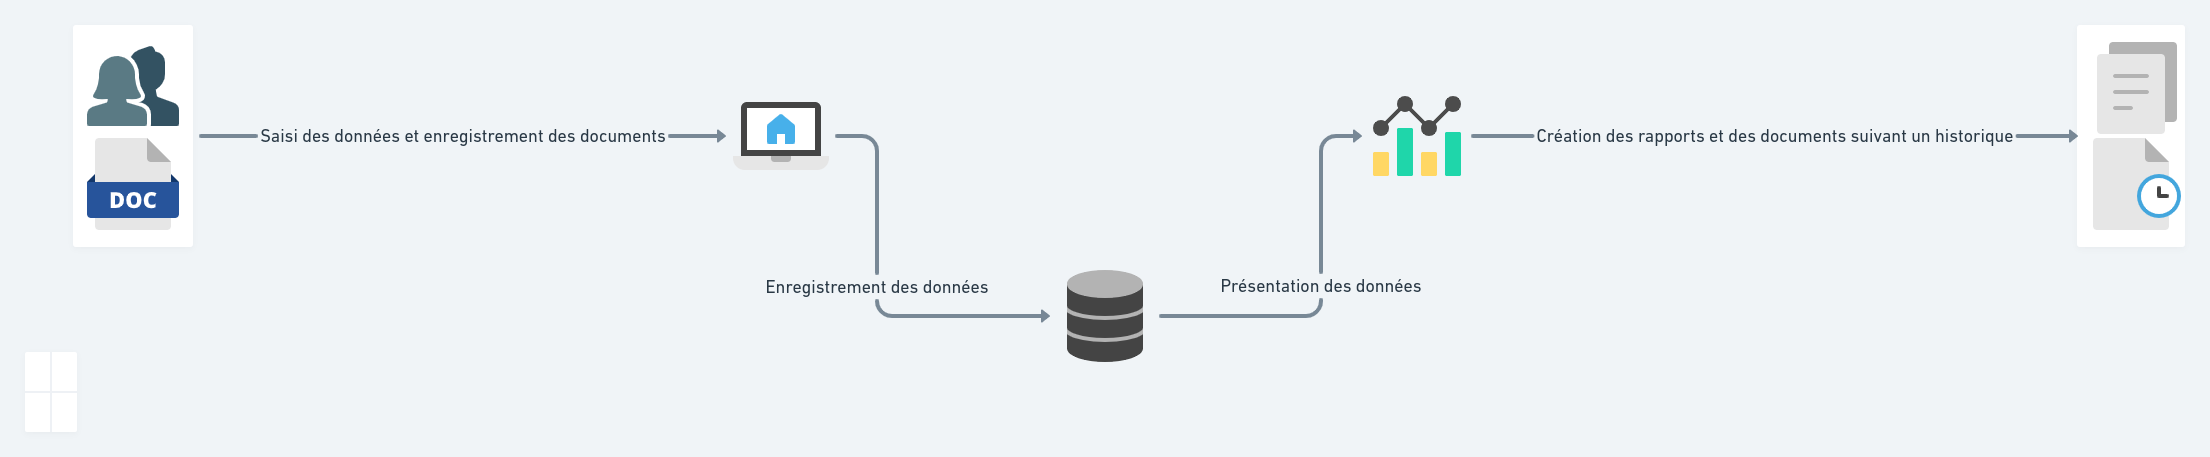
\includegraphics[scale=0.2]{images/pre-descip-projet.png}}
			\caption{Description préliminaire du projet}
		\end{center}
	\end{figure}
	\subsection{Étude de l’existant}

	Après la recherche et des exemples similaire à notre projet, on a
	trouvé une diversité des sites web et des applications dédiées à la gestion et
	au suivi.
	À titre d'exemple on peut considérer l'application \textbf{\large Ecan}:

	Généralement, les applications similaires sont des applications qui
	aide à la gestion de donnée et des ressources, et la prise des décisions.
	L’application \emph{Environnement Canterbury (ECan)} fait partie du
	gouvernement local de la région de Canterbury en Nouvelle-Zélande. Ils ont
	utilisé la plate-forme \emph{Power
		(PowerApps, Microsoft Flow et Power BI)} pour gérer et rendre compte
	efficacement des projets d'eau douce et de ressources naturelles.

	D’après l'article intitulé Environnement Canterbury accélère le suivi
	des
	résultats avec \emph{la Power Platform} :
	« Environnement Canterbury travaille en partenariat avec les communautés
	de
	Canterbury pour promouvoir la gestion durable des ressources
	naturelles. Cela
	implique l'utilisation de méthodes innovantes, rentables et
	techniquement
	excellentes, et garantit que la prise de décision est basée sur des
	informations
	de la plus haute qualité. Ils travaillent sur des programmes de
	résultats
	environnementaux à long terme qui consistent en plusieurs étapes et
	projets
	connexes. ECan avait besoin d'une solution abordable qui offrirait une
	plus
	grande cohérence entre les projets, des niveaux de visibilité plus
	élevés et un
	accès plus rapide aux données ».
	\begin{figure}[H]
		\begin{center}
			\fbox{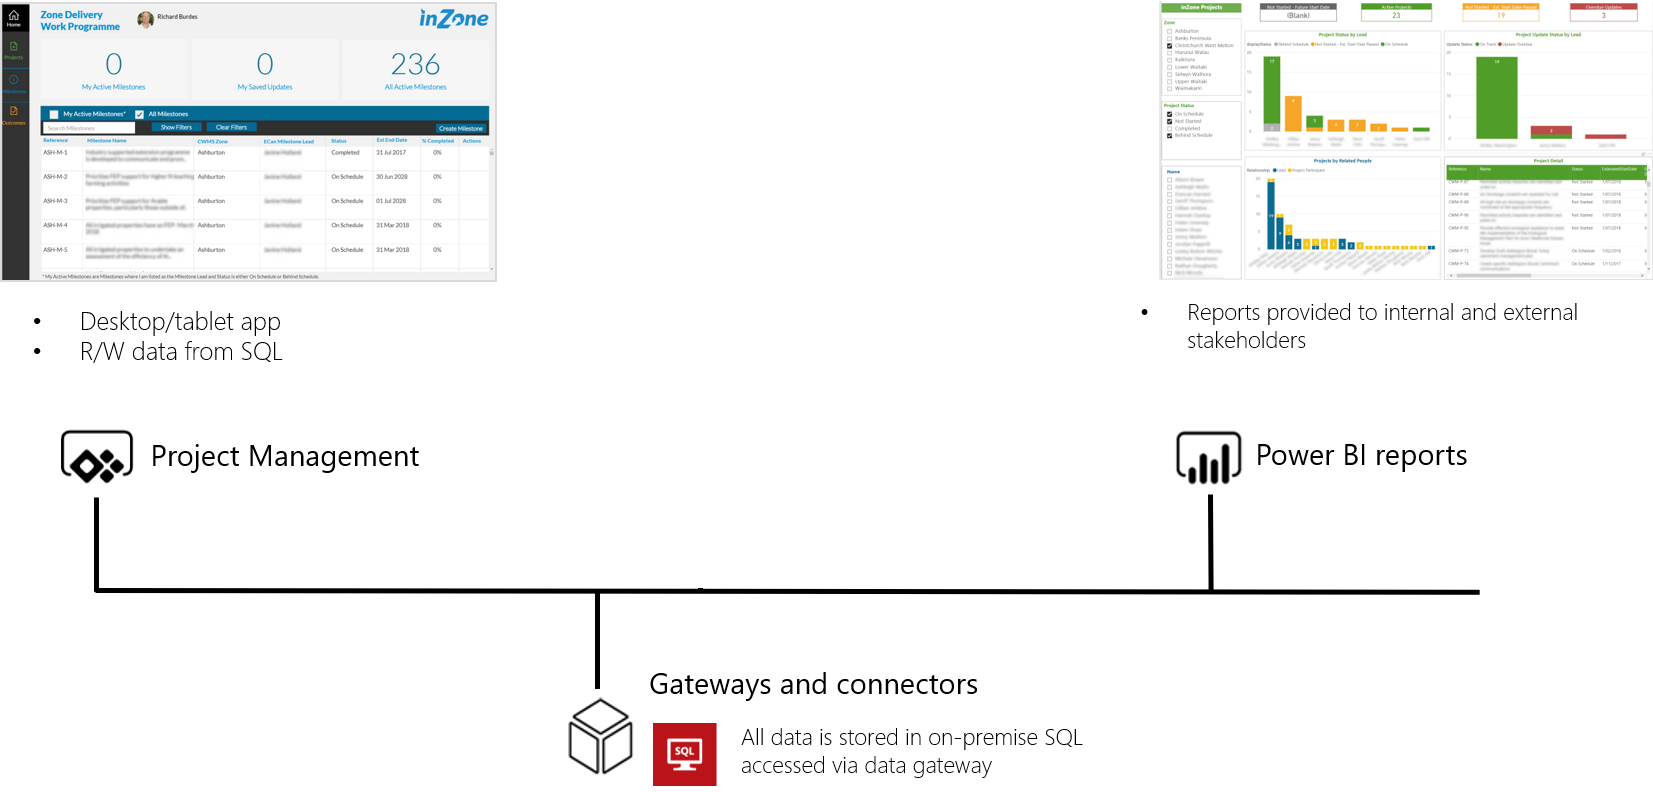
\includegraphics[scale=0.32]{images/example.png}}
			\caption{Exemple de Environnement Canterbury (ECan)}
		\end{center}
	\end{figure}
	\newpage
	\section{Spécification des besoins}

	\subsection{Spécification des acteurs}
	Vu que les informations gérées par cette application sont des informations confidentielles de l'état, l'application va avoir en général un seul acteur:
	L'administrateur est la personne chargée de charger les informations des différentes communes et de gérer leurs données, préparées par les différentes communes du Maroc.
	\subsection{Besoins fonctionnels}
	\begin{itemize}
		\item[•] Gestion des délégants et des délégataires: L'administrateur doit avoir
		      une section où il pourra gérer les délégants et les délégataires.
		\item[•] Gestion des contrats: Il doit avoir également la possibilité de gérer les contrats signés. En addition, il peut suivre les avenants et les révisions de chaque contrats. Ainsi que le status de chaque avenant ou révision.
		\item[•] Gestion des Avancements: L'application doit permettre de gérer les avancements semestriels des contrats. Aussi, consulter et suivre les changements apportés à chaque période.
		\item[•] Présentation des tableaux de bord: L'application doit présenter des données historisées de chaque contrats permettant de bien estimer la qualité de service en question et prendre les bonnes décisions.
		\item[•] Sauvegarde des fichiers sur un serveur WEB, et de sauvegarder en base de données le chemin de celui-ci. Généralement, cette solution est assez efficace, assez simple à mettre en œuvre.
	\end{itemize}
	\subsection{Les besoins non fonctionnels}
	Les besoins fonctionnels sont basiques pour un fonctionnement
	correcte et une réponse fiable aux besoins des utilisateurs, mais il y a des
	autres besoins qui tendent à améliorer la performance et la qualité de
	l'application pour une utilisation plus adéquate.
	\begin{itemize}
		\item[•] Fiabilité de la plateforme: L’application doit
		      fonctionner sans erreur.
		\item[•] Ergonomie, souplesse et confort d’utilisation: Pour
		      faciliter l’utilisation, notre plateforme doit offrir une interface unifiée,
		      conviviale et ergonomique.
		\item[•] Gain de temps: L'application doit optimiser les
		      traitements pour avoir un temps de réponse minimale.
		\item[•] Maintenabilité et sociabilité: La source de l'application doit être compréhensible
		      afin d’assurer son état évolutif et extensible par rapport aux besoins des utilisateurs. En outre, l’expérience des utilisateurs doit être meilleurs.
		\item[•] Sécurité: Notre plateforme doit  être très authentique en ce qui concerne les informations confidentielles des communes.
	\end{itemize}
	\section{Analyse fonctionnelle}
	Suivant à ce qui précède et d’après l’ensemble des documents communiqués par mes encadrants, j’ai essayé de créer une décomposition hiérarchique des fonctionnalités du projet.
	\begin{figure}[H]
		\begin{center}
			\fbox{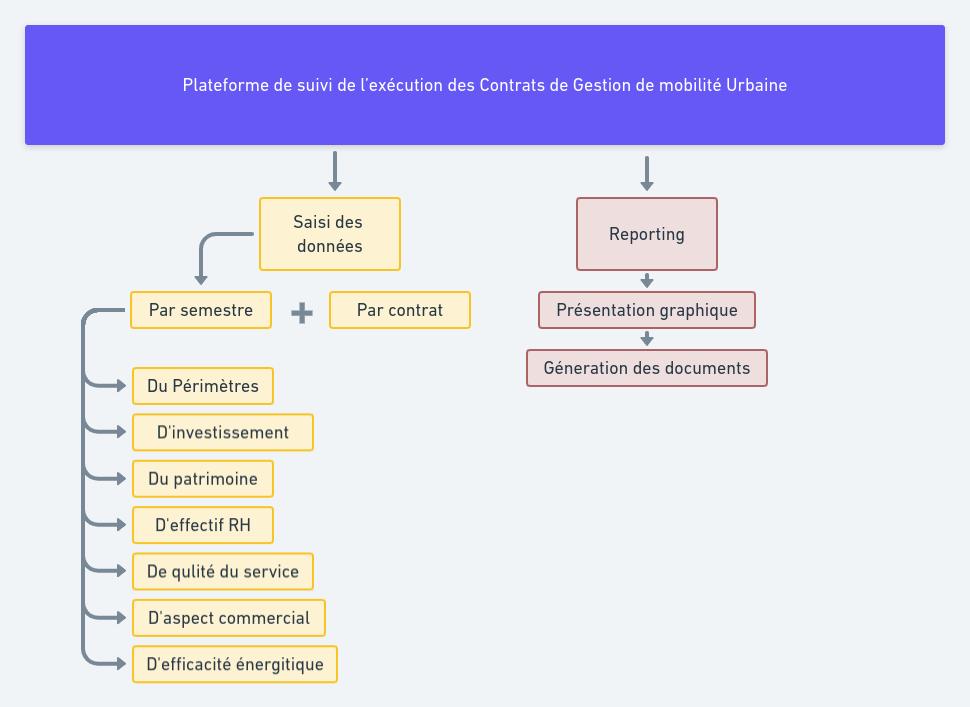
\includegraphics[scale=0.5]{images/WBS KPI.png}}
			\caption{Décomposition fonctionnelle du projet}
		\end{center}
	\end{figure}
	Ainsi, J'ai divisé le projet en deux parties fondamentales. En plus, on peut voir clairement les grandes fonctionnalités demandées dans cette application. Par conséquent, l'application peut être divisée en deux partie: partie saisi et partie reporting.
	\begin{itemize}
		\item[•] La partie saisi est la partie dans laquelle l'administrateur peut ajouter des délégants et des délégataires. En conséquences, il peut définir un contrat. Par ailleurs, le contrat définit peut avoir des mises à jour semestriels des informations qui le concerne.
		\item[•] La partie reporting est la partie qui concerne les tableaux de bords de l’application. Il doit bien présenter les informations saisîtes. En plus, il est préférables d'avoir la possibilité de générer des documents contenants les informations saisîtes.
	\end{itemize}
	\section{Analyse technique}
	La solution que je propose est une solution basée sur les données.
	Autrement dite, elle permet à son utilisateur d'interagir avec plusieurs
	informations. En outre, elle représente une solution spécialisée pour
	l'acquisition, la gestion et la présentation d'informations. Ainsi, le groupe du projet à proposer l'ensemble des outils suivants:
	\begin{figure}[H]
		\begin{center}
			\fbox{
\includegraphics[scale=0.41]{images/outilsDB.png}}
			\caption{Base de donnée SQL SERVER}
		\end{center}
	\end{figure}
	Microsoft SQL Server est un système de gestion
	de base de données relationnelle développé
	par Microsoft. En tant que serveur de base de
	données, il s'agit d'un produit logiciel dont la
	fonction principale est de stocker et de
	récupérer des données à la demande d'autres
	applications logicielles, qui peuvent
	s'exécuter sur le même ordinateur ou sur un
	autre ordinateur via un réseau.
	\begin{figure}[H]
		\begin{center}
			\fbox{
\includegraphics[scale=0.41]{images/outilsDEV.png}}
			\caption{Microsoft Power Apps}
		\end{center}
	\end{figure}
	Power Apps est un service permettant de créer
	et d'utiliser des applications professionnelles
	personnalisées qui se connectent à vos
	données et fonctionnent sur le Web et les
	appareils mobiles - sans le temps et les frais
	de développement de logiciels personnalisés.
	\begin{figure}[H]
		\begin{center}
			\fbox{
\includegraphics[scale=1.1]{images/outilsREP.png}}
			\caption{Microsft Power BI}
		\end{center}
	\end{figure}
	Power BI est un service d'analyse
	commerciale de Microsoft. Il vise à fournir des
	visualisations interactives et des capacités de
	business intelligence avec une interface
	suffisamment simple pour que les utilisateurs
	finaux puissent créer leurs propres rapports et
	tableaux de bord. Il fait partie de la plate-
	forme Microsoft Power.\\
	Suite à cette proposition le consultant technique a approuver ces choix. Ainsi la décision est prise d'utiliser ces technologies Microsoft afin de réaliser une application Low-Code pour la gestion des contrats de transport délégués.
	\section{Planification et démarche de travail}
	\subsection{Plan de travail prévu}
	Pour la bonne organisation des étapes du projet, j'ai proposé premièrement le plan suivant pour la réalisation de la plateforme demandée:
	\begin{figure}[H]
		\begin{center}
			\fbox{\includegraphics[scale=0.3]{images/GanttPrévu.png}}
			\caption{Plan de travail prévu du projet}
		\end{center}
	\end{figure}
	\subsection{Définition des Livrables}
	À la fin de chaque étape de la réalisation
	(section dans le diagramme de Gantt si-dessus),
	il est exigé d'avoir un livrable.
	Les livrables que nous proposons sont les suivants:
	\begin{table}[H]
		\begin{center}
			\begin{tabularx}{17.5cm}{|p{2cm}|X|}
				\hline
				\textbf{Étape} & \textbf{Livrable}                                                                                                                                                                  \\
				\hline
				Analyse        & Document de spécification décrivant le besoin, les fonctionnalités de la solution à implémenter, les technologies à utiliser, et toutes les contraints à respecter dans le projet. \\
				\hline
				Conception     & Document de conception qui donne une idée clair et global sur le projet.                                                                                                           \\
				\hline
				Réalisation    & Plateforme de suivi de l’exécution des contrats de gestion de mobilité urbaine.                                                                                                    \\
				\hline
			\end{tabularx}
			\caption{Livrables prévus de projet}
		\end{center}
	\end{table}
	\subsection{Les acteurs du projet}
	\begin{itemize}
		\item[•] \textbf{L’équipe du travail:} La tâche de la conception et de développement de l’application est assigné à moi.
		\item[•] \textbf{Le product owner:} Qui est ici la \textbf{DGST} représenté par monsieur Labiz Ibrahim. Il tient le rôle de définir les fonctionnalités et de s’assurer du bon fonctionnement du projet.
		\item[•] \textbf{Le SCRUM master:} Mon encadrante, Mme. Insaf Talhaoui a tenu ce rôle, en veillant sur la réalisation du projet.
	\end{itemize}
	\subsection{Les sprints du projet}
	Pour le bon déroulement du projet, le travail sera découpé en sprint. Ces sprints sont établi à l’aide du product backLog tout en respectant la priorité des différents modules. À la fin de chaque sprint, on aura un livrable qui sera examiné par le Product Owner afin de planifier les modifications et les évolutions à effectuer dans le sprint suivant. La planification du projet selon les sprints et comme suit :
	\begin{table}[H]
		\begin{center}
			\begin{tabularx}{17.5cm}{|p{2cm}|p{2cm}|X|}
				\hline
				\textbf{Numéro} & \textbf{Durée} & \textbf{Description}                                                                            \\
				\hline
				1               & 2 semaines     & Réalisation et connexion à la base de donnée.                                                   \\
				\hline
				2               & 2 semaines     & Création de la partie gestion des contrats et d'un référence des délégants et des délégataires. \\
				\hline
				3               & 2 semaines     & Création de la partie suivis des contrats.                                                      \\
				\hline
				4               & 2 semaines     & Réalisation des tableaux de bords demandés.                                                     \\
				\hline
			\end{tabularx}
			\caption{Les Sprints du projet}
		\end{center}
	\end{table}
	\subsection{Mode de travail}
	Afin de réaliser le projet, on doit définir un mode de travail convenable. Le mode de
	travail que je propose est le mode agile en utilisant SCRUM. Puisque je travaille
	dans un environnement où je garde un contact continue avec le Product Owner. En
	plus, je cherche à avoir une communication efficace avec le client pour le
	satisfaire en lui livrant fréquemment un état d'avancement tangible.
	D'ailleurs, le temps est un facteur important dans ce projet. De ce fait, il faut sentir
	l’avancement quotidienne du projet. En addition, il faut faire attention continue à
	l’excellence technique, à une meilleure conception et produire uniquement ce qui est
	nécessaire dans les meilleurs délais. Pour ce faire j'ai utilisé la plateforme Trello. Ainsi, on présente le tableau suivant basée sur le modèle kanban pour l'organisation des tâches et des livrables:
	\begin{figure}[H]
		\begin{center}
			\fbox{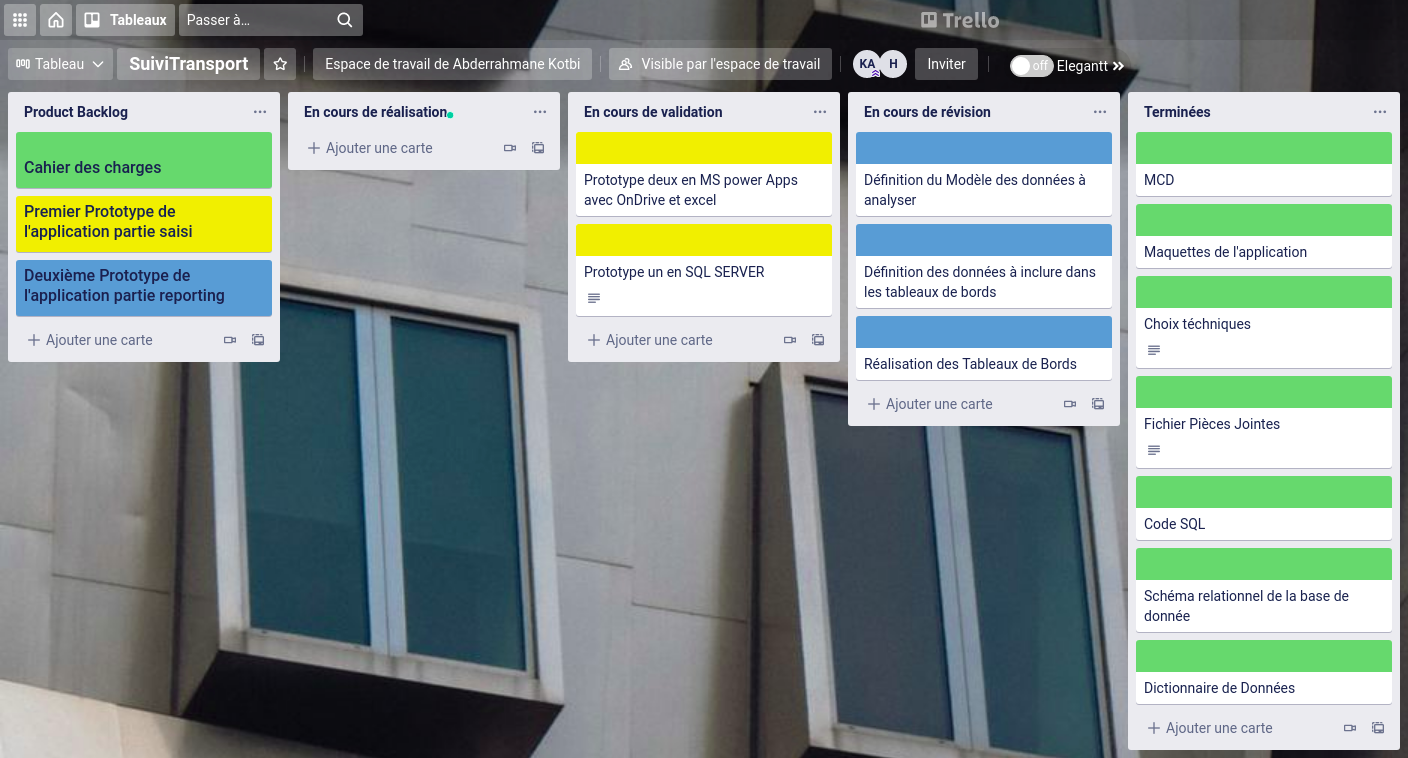
\includegraphics[scale=0.37]{images/trello.png}}
			\caption{Modèle Kanban du projet}
		\end{center}
	\end{figure}
	\section{Récapitulatif}
	Dans ce chapitre, j'ai déterminé les acteurs principaux dans ce projet ainsi que leur
	besoin. L'étude élaborée serai ma base de travail par la suite, à
	savoir: la conception et la réalisation de notre projet. Dans le chapitre suivant je vais
	exposer ma vue conceptuelle vis-à-vis au projet.
	\begin{figure}[H]
		\begin{center}
			\fbox{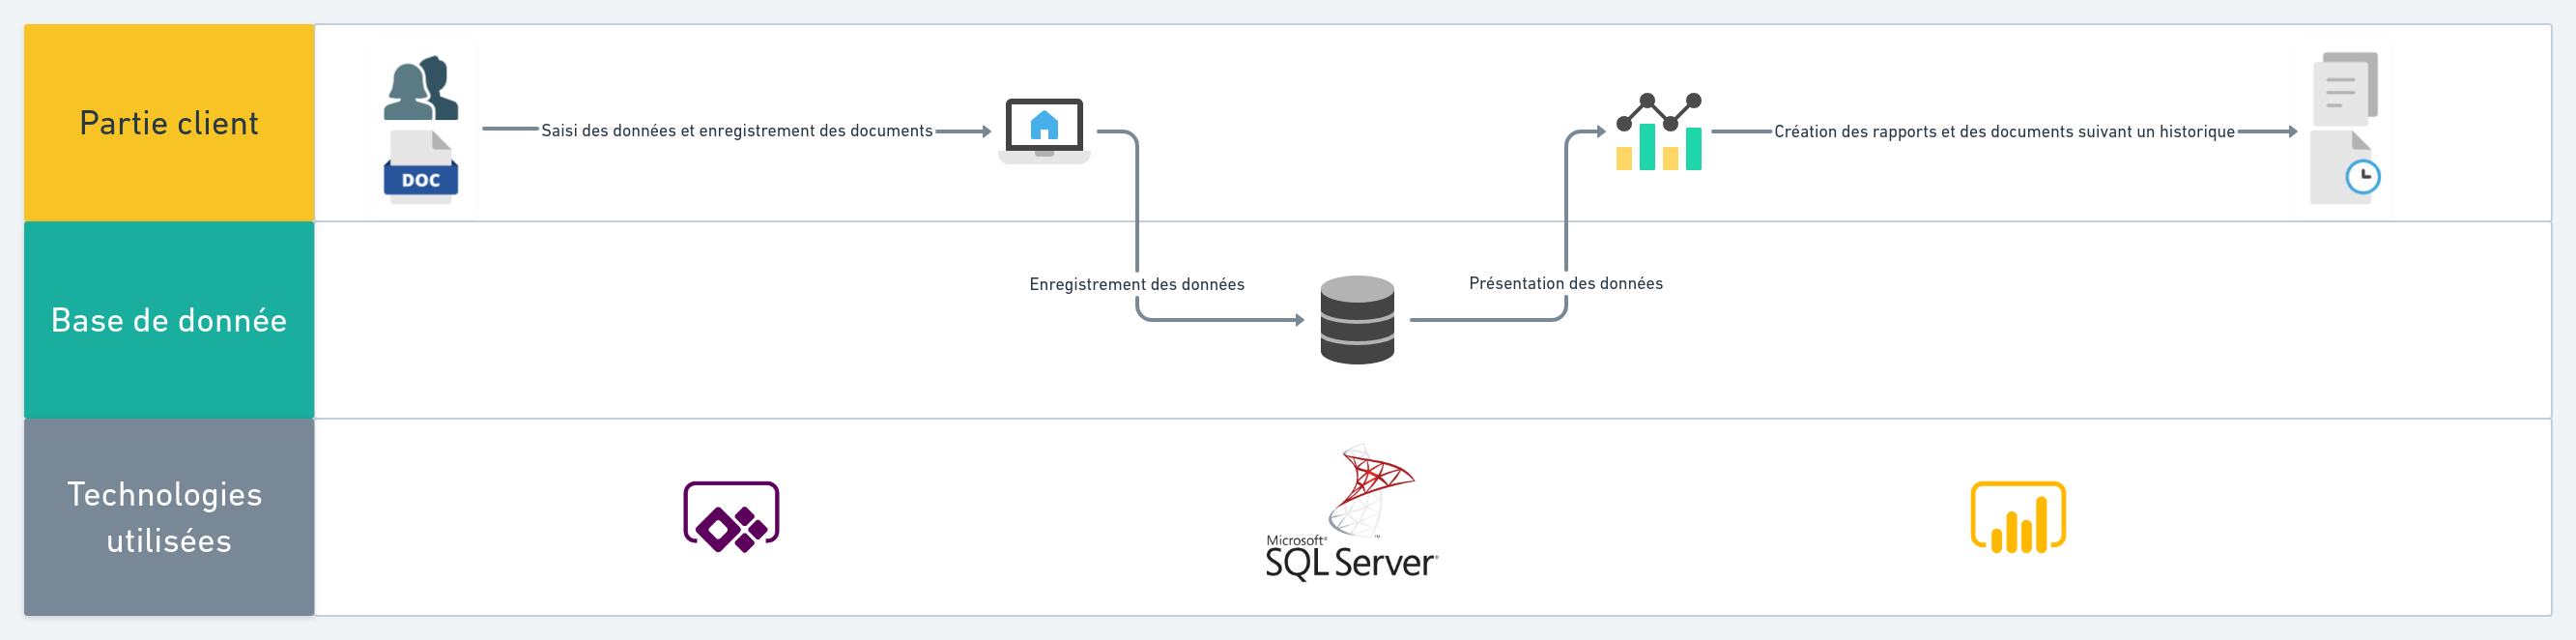
\includegraphics[scale=0.19]{images/KDI.png}}
			\caption{Description générale du projet}
		\end{center}
	\end{figure}
	\chapter{Étude conceptuelle}
	\fancyhead[R]{\textbf{Chapitre \thechapter: Étude conceptuelle}}
	\fancyhead[L]{\hspace*{5cm}}
	Cette partie est très importante dans le cycle de vie du projet. Théoriquement, toute la fondation du projet a été construite dans cette base, par la suite, il ne reste que la mise en œuvre.
	\section{Étude des données}
	\subsection{Règles de gestion recensées}
	Au cours de la réalisation du projet, j'ai vu qu’un ensemble de règles de gestion sont à respecter afin d'assurer la bonne satisfaction du besoin et le bon fonctionnement du système. Quant à ce projet j'ai proposé l’ensemble des règles suivantes:
	\begin{itemize}
		\item[•] L'administrateur de système doit demander l’accès au système pour recevoir les informations de son compte de part du directeur de l'espace Office 365 \textbf{DYN IT}.
		\item[•] L'administrateur doit choisir un contrat pour accéder et gérer ses informations.
		\item[•] L'administrateur doit voir toujours les informations d'entête d'un contrat sélectionné.
		\item[•] L'administrateur doit choisir un contrat et une période pour accéder et gérer les informations reliées aux avancements semestriels.
		\item[•] L'administrateur doit avoir un référentiel des délégants et des délégataires.
		\item[•] L'administrateur doit avoir la possibilité de modifié le référentiel des délégants ou des délégataires.
		\item[•] L'administrateur doit avoir la possibilité d'accéder à des tableaux de bord modifiable selon le contrat et/ou la période.
		\item[•] L'administrateur doit avoir la possibilité de générer des rapports d'un contrat et/ou une période sélectionnée.
	\end{itemize}
	\subsection{Dictionnaire des données}
	Pour bien comprendre les données traitées dans ce projet, j'ai obtenu plusieurs documents de suivi et un exemple de contrat de gestion déléguée. Ainsi, j'ai proposé le dictionnaire des données suivant. Ce dernier est divisées en plusieurs tableaux qui sont classées dans trois catégories:
	\begin{itemize}
		\item[•] Les données d'entête: Ils représentes les informations qui définissent un contrat. Certes, ils peuvent être gérer, mais ils ne dépendent pas des périodes. Ils ne peuvent pas être changées sauf dans le cadre d'une révision ou d'un avenant.
		\item[•] Les données des référentiels: Ils représentes les informations qui ne dépendent ni du contrat et ni de la période. En effet, il peuvent être inclus dans la définitions d'un contrat.
		\item[•] Les données d'avancements: Ils représentes les informations qui dépendent du contrat et de la période.
	\end{itemize}

	\subsubsection{• Les données d'entête}

	Cette catégorie groupe les données des contrats, des révisions, des avenants, des tarifs, etc.

	\begin{table}[H]
		\begin{center}
			\begin{tabularx}{17.5cm}{|p{3.5cm}|X|p{3.5cm}|}
				\hline
				\textbf{Attribut}    & \textbf{Signification}                                        & \textbf{Exemple}    \\
				\hline
				NumContrat           & Numéro du contrat                                             & 45858               \\
				\hline
				LibelleContrat       & Libellé du contrat                                            & ALBAIDA             \\
				\hline
				DateDemarrageContrat & Date de démarrage du contrat                                  & 01/11/2019          \\
				\hline
				DateFinContrat       & Date du fin du contrat                                        & 01/11/2027          \\
				\hline
				DateVisa             & Date visa                                                     & 01/06/2019          \\
				\hline
				DureeContrat         & Durée du contrat                                              & 10 ans              \\
				\hline
				Delegant             & Nom du délégant                                               & Commune Tanger      \\
				\hline
				Delegataire          & Nom du délégataire                                            & ALSA Tanger         \\
				\hline
				Autre Partenaire     & Nom d'un partenaire (autre que le délégant et le délégataire) & Coopération El-Amal \\
				\hline
				NumAvenant           & Numéro d'avenant                                              & 5245                \\
				\hline
				LibelleAvenant       & Libellé d'avenant                                             &                     \\
				\hline
				DateAvenant          & Date d'avenant                                                & 01/06/2023          \\
				\hline
				MotifAvenant         & Motif d'avenant                                               &                     \\
				\hline
				Status               & Status d'avenant                                              & Actif/ Non Actif    \\
				\hline
				NumRevision          & Numéro de révision                                            & 2336                \\
				\hline
				LibelleRevision      & Libellé de révision                                           &                     \\
				\hline
				DateRevision         & Date de révision                                              & 01/01/2026          \\
				\hline
				MotifRevision        & Motif de la révision                                          &                     \\
				\hline
			\end{tabularx}
			\caption{Table d'entête}
		\end{center}
	\end{table}
	\begin{table}[H]
		\begin{center}
			\begin{tabularx}{17.5cm}{|p{6.5cm}|X|p{2.1cm}|}
				\hline
				\textbf{Attribut}                    & \textbf{Signification}                                       & \textbf{Exemple} \\
				\hline
				NumCommunesDesservies                & Nombre de communes desservies                                & 10               \\
				\hline
				Population                           & Population                                                   & 100252           \\
				\hline
				LongueurReseau                       & Longueur du réseau                                           & 200 Km           \\
				\hline
				LongueurLignesUrbaines               & Longueur des lignes urbaines                                 & 130 Km           \\
				\hline
				LongueurLignesPeripheriques          & Longueur des lignes périphériques                            & 70km             \\
				\hline
				NombreLignes                         & Nombre des lignes                                            & 24               \\
				\hline
				PrixMinTarifScolaire                 & Prix minimal de tarif scolaire                               & 3 Dhs            \\
				\hline
				PrixMaxTarifScolaire                 & Prix maximal de tarif scolaire                               & 6 Dhs            \\
				\hline
				PrixMinTarifNormal                   & Prix minimal de tarif normal                                 & 4 Dhs            \\
				\hline
				PrixMaxTarifNormal                   & Prix maximal de tarif normal                                 & 5 Dhs            \\
				\hline
				PrixMinTarifConvention               & Prix maximal de tarif convention                             & 5 Dhs            \\
				\hline
				PrixMaxTarifConvention               & Prix maximal de tarif convention                             & 7 Dhs            \\
				\hline
				ValeurInvestissementContractuelDN    & Valeur d'investissement contractuel de délégant              & 150000 Dhs       \\
				\hline
				NombreBusContractuelDN               & Nombre des bus contractuel de délégant                       & 50               \\
				\hline
				NombreAbriBusContractuelDN           & Nombre des abris bus contractuel de délégant                 & 15               \\
				\hline
				NombreArretContractuelDN             & Nombre des arrêts contractuel de délégant                    & 150              \\
				\hline
				NombreAireStationnementContractuelDN & Nombre des aires de stationnement contractuel de délégant    & 10               \\
				\hline
				ValeurInvestissementContractuelDT    & Valeur d'investissement contractuelle de délégataire         & 100000 Dhs       \\
				\hline
				NombreBusContractuelDT               & Nombre des bus contractuel de délégataire                    & 45               \\
				\hline
				NombreAbriBusContractuelDT           & Nombre des abris bus contractuel de délégataire              & 10               \\
				\hline
				NombreArretContractuelDT             & Nombre des arrêts contractuel de délégataire                 & 120              \\
				\hline
				NombreAireStationnementContractuelDT & Nombre des aires de stationnement contractuel de délégataire & 7                \\
				\hline
			\end{tabularx}
			\caption{Suite 1 de la table d'entête}
		\end{center}
	\end{table}
	\begin{table}[H]
		\begin{center}
			\begin{tabularx}{17.5cm}{|p{6cm}|X|p{1.6cm}|}
				\hline
				\textbf{Attribut}                    & \textbf{Signification}                                                                                          & \textbf{Exemple} \\
				\hline
				ValeurInvestissementContractuelleAT  & Valeur d'investissement contractuelle des autres partenaires (autre que le délégants et le délégataire)         & 90000 Dhs        \\
				\hline
				NombreBusContractuelAT               & Nombre des bus contractuel des autres partenaires (autre que le délégants et le délégataire)                    & 30               \\
				\hline
				NombreAbriBusContractuelAT           & Nombre des abris bus contractuel des autres partenaires (autre que le délégants et le délégataire)              & 7                \\
				\hline
				NombreArretContractuelAT             & Nombre des arrêts contractuel des autres partenaires (autre que le délégants et le délégataire)                 & 80               \\
				\hline
				NombreAireStationnementContractuelAT & Nombre des aires de stationnement contractuel des autres partenaires (autre que le délégants et le délégataire) & 0                \\
				\hline
			\end{tabularx}
			\caption{Suite 2 de la table d'entête}
		\end{center}
	\end{table}

	\subsubsection{Les données des référentiels}

	Cette catégorie groupe les données des délégataires, des délégants et des communes.

	\begin{table}[H]
		\begin{center}
			\begin{tabularx}{17.5cm}{|p{3cm}|p{3cm}|X|}
				\hline
				\textbf{Attribut} & \textbf{Signification} & \textbf{Exemple}                                       \\
				\hline
				NomDelegant       & Nom du délégant        & Établissement de Coopération Intercommunal  "Al Baida" \\
				\hline
			\end{tabularx}
			\caption{Référentiel des délégants}
		\end{center}
	\end{table}

	\begin{table}[H]
		\begin{center}
			\begin{tabularx}{17.5cm}{|p{3cm}|p{3cm}|X|}
				\hline
				\textbf{Attribut} & \textbf{Signification} & \textbf{Exemple}    \\
				\hline
				NomDelegataire    & Nom du délégataire     & Société ALSA Tanger \\
				\hline
			\end{tabularx}
			\caption{Référentiel des délégataires}
		\end{center}
	\end{table}

	\newpage
	\subsubsection{Les données des avancements}

	Cette catégorie groupe les données d'effectif personnel, des investissements, des matériaux roulants et fixes, etc...


	\begin{table}[H]
		\begin{center}
			\begin{tabularx}{17.5cm}{|p{2.5cm}|X|p{2.5cm}|}
				\hline
				\textbf{Attribut} & \textbf{Signification}                                                                              & \textbf{Exemple} \\
				\hline
				numcontrat        & Numéro du Contrat                                                                                   & 25462            \\
				\hline
				numavenant        & Numéro d'avenant                                                                                    & 14528            \\
				\hline
				numrevision       & Numéro de révision                                                                                  & 1552             \\
				\hline
				valeur\_delegant  & Somme investi par le délégant                                                                      & 900000 Dhs       \\
				\hline
				abri\_delegant    & Nombre des abris bus de délégant                                                                    & 6                \\
				\hline
				arret\_delegant   & Nombre des arrêts de délégant                                                                       & 7                \\
				\hline
				bus\_delegant     & Nombre des bus de délégant                                                                         & 50               \\
				\hline
				air\_delegant     & Nombre des aires de stationnement de délégant                                                       & 30               \\
				\hline
				air\_delegataire  & Nombre des aires de stationnement de délégataire                                                    & 25               \\
				\hline
				valeur\_autre     & Somme investi par les autres partenaires (autre que le délégants et le délégataire)                & 800000 Dhs       \\
				\hline
				abri\_autre       & Nombre des abris bus des autres partenaires (autre que le délégants et le délégataire)              & 3                \\
				\hline
				arret\_autre      & Nombre des arrêts des autres partenaires (autre que le délégants et le délégataire)                 & 25               \\
				\hline
				bus\_autre        & Nombre des bus des autres partenaires (autre que le délégants et le délégataire)                    & 20               \\
				\hline
				air\_autre        & Nombre des aires de stationnement des autres partenaires (autre que le délégants et le délégataire) & 15               \\
				\hline
				datedemiseajour   & Date de mise à jour                                                                                 & 16/04/2021       \\
				\hline
				periode           & Année/semestre                                                                                      & 2020/S1          \\
				\hline
			\end{tabularx}
			\caption{Table d'investissements réalisés}
		\end{center}
	\end{table}

	\begin{table}[H]
		\begin{center}
			\begin{tabularx}{17.5cm}{|X|X|p{2.5cm}|}
				\hline
				\textbf{Attribut}                          & \textbf{Signification}                     & \textbf{Exemple} \\
				\hline
				numcontrat                                 & Numéro du Contrat                          & 25462            \\
				\hline
				numavenant                                 & Numéro d'avenant                           & 14528            \\
				\hline
				numrevision                                & Numéro de révision                         & 1552             \\
				\hline
				abris\_bus\_nombre                         & Nombre des abris bus                       & 15               \\
				\hline
				abris\_bus\_age moyen                      & Âge moyen de bus                           & 5 ans            \\
				\hline
				abris\_bus\_satisfaction                   & Satisfaisante des abris bus                 & 76\%             \\
				\hline
				abris\_bus\_capacité totale                & Capacité totale des abris bus              & 30 personnes     \\
				\hline
				arrêts\_nombre                             & Nombre des arrêts                          & 50               \\
				\hline
				arrêts\_age moyen                          & Âge moyen des arrêts                       & 5 ans            \\
				\hline
				arrêts\_satisfaction                       & Satisfaisante des arrêts                    & 80\%             \\
				\hline
				arrêts\_capacité\_totale                   & Capacité totale des arrêts                 & 15 personnes     \\
				\hline
				ateliers\_nombre                           & Nombre des ateliers                        & 3                \\
				\hline
				atelier\_age\_moyen                        & Âge moyen des ateliers                     & 15 ans           \\
				\hline
				ateliers\_satisfaction                     & Satisfusance des ateliers                  & 70\%             \\
				\hline
				ateliers\_capacité\_totale                 & Capacité totale des ateliers               & 100 personnes    \\
				\hline
				aires\_de\_stationnement\_nombres          & Nombre des aires de stationnement          & 45               \\
				\hline
				aires\_de\_stationnement\_age\_moyen       & Âge moyen des aires de stationnement       & 7 ans            \\
				\hline
				aires\_de\_stationnement\_satisfaction     & Satisfusance des aires de stationnement    & 77\%             \\
				\hline
				aires\_de\_stationnement\_capacité\_totale & Capacité totale des aires de stationnement & 70 personnes     \\
				\hline
				guichet\_nombre                            & Nombre des guichets                        & 50 guichets      \\
				\hline
				guichet\_age\_moyen                        & Âge moyen des guichets                     & 7 ans            \\
				\hline
				guichet\_capacité\_totale                  & Capacité totale des guichets               & 10 personnes     \\
				\hline
				guichet\_satisfaction                      & Satisfusance des guichets                  & 63\%             \\
				\hline
				datedemiseajour                            & Date de mise à jour                        & 16/04/2021       \\
				\hline
				periode                                    & Année/semestre                             & 2020/S1          \\
				\hline
			\end{tabularx}
			\caption{Table des matériaux fixes}
		\end{center}
	\end{table}

	\begin{table}[H]
		\begin{center}
			\begin{tabularx}{17.5cm}{|p{6cm}|X|p{2.5cm}|}
				\hline
				\textbf{Attribut}                 & \textbf{Signification}                           & \textbf{Exemple} \\
				\hline
				numcontrat                        & Numéro du Contrat                                & 25462            \\
				\hline
				numavenant                        & Numéro d'avenant                                 & 14528            \\
				\hline
				numrevision                       & Numéro de révision                               & 1552             \\
				\hline
				Bus\_standard\_nombre             & Nombre des bus standard                          & 50               \\
				\hline
				bus\_standard\_age\_moyen         & Âge moyen des bus standard                       & 7 ans            \\
				\hline
				bus\_standard\_km\_parcourus      & Nombre des Km parcourus des bus standard         & 80 Km            \\
				\hline
				bus\_articulé\_nombre             & Nombre des bus articulés                         & 20               \\
				\hline
				bus\_articulé\_age\_moyen         & Âge moyen des bus articulés                      & 7 ans            \\
				\hline
				bus\_articulés\_km\_parcourus     & Nombre des Km parcourus des bus articulés        & 10500 Km         \\
				\hline
				bus\_éléctrique\_nombre           & Nombre des bus électriques                       & 10               \\
				\hline
				bus\_éléctrique\_age\_moyen       & Âge moyen des bus électriques                    & 10 ans           \\
				\hline
				bus\_éléctrique\_km\_parcourus    & Nombre des Km parcourus des bus électriques      & 80000 Km         \\
				\hline
				bus\_sites\_propres\_nombre        & Nombre des bus des sites propres                  & 15               \\
				\hline
				bus\_sites\_propres\_age\_moyen    & Âge moyen des bus des sites propres               & 15 ans           \\
				\hline
				bus\_sites\_propres\_km\_parcourus & Nombre des Km parcourus des bus des sites propres & 70000 Km         \\
				\hline
				datedemiseajour                   & Date de mise à jour                              & 16/04/2021       \\
				\hline
				periode                           & Année/semestre                                   & 2020/S1          \\
				\hline
			\end{tabularx}
			\caption{Table des matériaux circulants}
		\end{center}
	\end{table}

	\begin{table}[H]
		\begin{center}
			\begin{tabularx}{17.5cm}{|p{4cm}|X|p{2.5cm}|}
				\hline
				\textbf{Attribut}          & \textbf{Signification}                                                                                      & \textbf{Exemple} \\
				\hline
				numcontrat                 & Numéro du Contrat                                                                                           & 25462            \\
				\hline
				numavenant                 & Numéro d'avenant                                                                                            & 14528            \\
				\hline
				numrevision                & Numéro de révision                                                                                          & 1552             \\
				\hline
				PQM                        & Plan de Maintenance Qualité                                                                                 & oui              \\
				\hline
				Réclamation                & Réclamations des usagers                                                                                    & 152              \\
				\hline
				Equipements\_points\_arrêt & Équipements des points d'arrêt                                                                              & Poteaux          \\
				\hline
				SAEV                       & Système d'information de type Systèmes d'Aide à l'Exploitation et
				à l'Information Voyageurs  & non                                                                                                                            \\
				\hline
				SysGeo                     & Système de géolocalisation                                                                                  & oui              \\
				\hline
				AdresseSTR                 & Site internet et information disponible en temps réel (adresse)                                             & non              \\
				\hline
				AdressedescpSTR            & Site internet et information disponible  en temps réel (Description d'adresse)                                & oui              \\
				\hline
				ReseauSTR                  & Site internet et information disponible  en temps réel (Informations Statiques sur le réseau)               & oui              \\
				\hline
				ReseaudescpSTR             & Site internet et information disponible  en temps réel (Description des informations Statiques sur le réseau) & non              \\
				\hline
				HoraireServiceSTR          & Site internet et information disponible  en temps réel (Horaire du services)                                & oui              \\
				\hline
				HoraireServicedescpSTR     & Site internet et information disponible  en temps réel (Description d'horaire du services)                    & oui              \\
				\hline
				PerturbationsSTR           & Site internet et information disponible  en temps réel (Informations sur les perturbations)                 & oui              \\
				\hline
				PerturbationsdescpSTR      & Site internet et information disponible  en temps réel (Description des informations sur les perturbations)   & oui              \\
				\hline
				TarifSTR                   & Site internet et information disponible  en temps réel (Tarifs appliqués)                                   & non              \\
				\hline
				TarifdescpSTR              & Site internet et information disponible  en temps réel (Description des tarifs appliqués)                   & oui              \\
				\hline
				VenteSTR                   & Site internet et information disponible  en temps réel(Vente en ligne)                                      & non              \\
				\hline
				VentedescpSTR              & Site internet et information disponible  en temps réel(Description des ventes en ligne)                     & oui              \\
				\hline
			\end{tabularx}
			\caption{Table de la qualité des services}
		\end{center}
	\end{table}
	\begin{table}[H]
		\begin{center}
			\begin{tabularx}{17.5cm}{|p{4cm}|X|p{2.5cm}|}
				\hline
				\textbf{Attribut}                       & \textbf{Signification}                                                 & \textbf{Exemple} \\
				\hline
				CorrespondanceSTR                       & Site internet et information disponible en temps réel (correspondance) & oui              \\
				\hline
				CorrespondancedescpSTR                  & Site internet et information disponible en temps
				réel (Description de la correspondance) & oui                                                                                       \\
				\hline
				IntermodalieSTR                         & Site internet et information disponible en temps réel intermodalité    & oui              \\
				\hline
				IntermodaliedescpSTR                    & Site internet et information disponible en temps
				réel (Description d'intermodalité)      & oui                                                                                       \\
				\hline
				wifi                                    & wifi embarqué                                                          & oui              \\
				\hline
				VideoSurveillance                       & Vidéo surveillance embarquée                                           & oui              \\
				\hline
				CentreAppel                             & Centre d'appel                                                         & oui              \\
				\hline
				datedemiseajour                         & Date de mise à jour                                                    & 16/04/2021       \\
				\hline
				periode                                 & Année/semestre                                                         & 2020/S1          \\
				\hline
			\end{tabularx}
			\caption{Suite de la table de la qualité des services}
		\end{center}
	\end{table}

	\begin{table}[H]
		\begin{center}
			\begin{tabularx}{17.5cm}{|p{4cm}|X|p{2cm}|}
				\hline
				\textbf{Attribut}    & \textbf{Signification}                           & \textbf{Exemple} \\
				\hline
				numcontrat           & Numéro du Contrat                                & 25462            \\
				\hline
				numavenant           & Numéro d'avenant                                 & 14528            \\
				\hline
				numrevision          & Numéro de révision                               & 1552             \\
				\hline
				NumVoyJrS            & Nombre moyen de voyageurs/jour  sur un semestre  & 15023            \\
				\hline
				NumPVJrS             & Nombre moyen place vide /jour  sur un semestre   & 1252             \\
				\hline
				VoyageurTotalS       & Total annuel des voyageurs  sur un semestre      & 1252535          \\
				\hline
				TicketsVendusT       & Tickets vendus/semestre totale                   & 1250535          \\
				\hline
				TicketsVendusSc      & Tickets vendus/semestre tarif scolaire           & 125325           \\
				\hline
				TicketsVendusN       & Tickets vendus/semestre tarif normal             & 925634           \\
				\hline
				TicketsVendusC       & Tickets vendus/semestre tarif conventions        & 65828            \\
				\hline
				KmParTS              & Km parcourus/semestre totale semestriel parcouru & 152360 Km        \\
				\hline
				KmParMoyenS          & Km parcourus/semestre moyenne par ligne          & 1253 Km          \\
				\hline
				KmParMoyenSTrajL     & Km parcourus/semestre trajet le plus long        & 10535 Km         \\
				\hline
				KmParMoyenSTrajCourt & Km parcourus/semestre trajet le plus court       & 1253 Km          \\
				\hline
				KmParMoyenSTempsMax  & Km parcourus/semestre temps max trajet           & 8526 Km          \\
				\hline
				KmParMoyenSTempsMin  & Km parcourus/semestre temps min trajet           & 4253 Km          \\
				\hline
			\end{tabularx}
			\caption{Table des aspects commerciaux}
		\end{center}
	\end{table}
	\begin{table}[H]
		\begin{center}
			\begin{tabularx}{17.5cm}{|p{4cm}|X|p{2cm}|}
				\hline
				\textbf{Attribut} & \textbf{Signification}                                            & \textbf{Exemple} \\
				\hline
				Frequence         & Fréquence moyenne de passage unité/heure                          & 20               \\
				\hline
				Vitesse           & Vitesse commerciale moyenne Durée moyenne des trajets bus         & 60 Km/h          \\
				\hline
				Ponctualite       & Ponctualité Écart moyen entre horaire contractuel et horaire réel & 60\%             \\
				\hline
				TauxRemplissage   & Taux moyen de remplissage                                         & 80\%             \\
				\hline
				TauxTransVide     & Taux de transport à vide                                          & 15\%             \\
				\hline
				Depart            & Horaires du départ du service                                     & 05:00            \\
				\hline
				HeureFin          & Horaires de fin du service                                        & 11:00            \\
				\hline
				Pannes            & Pannes des bus sur la voie publique                               & 200              \\
				\hline
				Accidents         & Accidents de circulation des bus                                  & 132              \\
				\hline
				DélaiEva          & Délai moyen d'évacuation des véhicules en panne                   & 25 min           \\
				\hline
				datedemiseajour   & Date de mise à jour                                               & 16/04/2021       \\
				\hline
				periode           & Année/semestre                                                    & 2020/S1          \\
				\hline
			\end{tabularx}
			\caption{Suite de la table des aspects commerciaux}
		\end{center}
	\end{table}

	\begin{table}[H]
		\begin{center}
			\begin{tabularx}{17.5cm}{|p{4cm}|X|p{3cm}|}
				\hline
				\textbf{Attribut}   & \textbf{Signification}                                      & \textbf{Exemple} \\
				\hline
				numcontrat          & Numéro du Contrat                                           & 25462            \\
				\hline
				numavenant          & Numéro d'avenant                                            & 14528            \\
				\hline
				numrevision         & Numéro de révision                                          & 1552             \\
				\hline
				ConsommationMoyStd  & Consommation moyenne par km et par type de bus standard     & 15263 tonnes     \\
				\hline
				ConsommationMoyArt  & Consommation moyenne par km et par type de bus articulé     & 15263 tonnes     \\
				\hline
				ConsommationMoyElec & Consommation moyenne par km et par type de bus électrique   & 15263 tonnes     \\
				\hline
				ConsommationMoySite & Consommation moyenne par km et par type de bus sites propres & 15263 tonnes     \\
				\hline
				ConsommationAnn     & Consommation carburant annuelle pour l'ensemble du parc     & 152630 tonnes    \\
				\hline
				ConsommationAnnEle  & Consommation totale en électricité annuelle                 & 1526003 Kwh      \\
				\hline
				Emissions           & Émissions Carbone  Co2                                      & 15263 tonnes     \\
				\hline
				datedemiseajour     & Date de mise à jour                                         & 16/04/2021       \\
				\hline
				periode             & Année/semestre                                              & 2020/S1          \\
				\hline
			\end{tabularx}
			\caption{Table de l’efficacité énergétique}
		\end{center}
	\end{table}

	\begin{table}[H]
		\begin{center}
			\begin{tabularx}{17.5cm}{|p{4cm}|X|p{2cm}|}
				\hline
				\textbf{Attribut}      & \textbf{Signification}           & \textbf{Exemple} \\
				\hline
				numcontrat             & Numéro du Contrat                & 25462            \\
				\hline
				numavenant             & Numéro d'avenant                 & 14528            \\
				\hline
				numrevision            & Numéro de révision               & 1552             \\
				\hline
				Conducteurs            & Nombre des conducteurs           & 200              \\
				\hline
				controleur             & Nombre des contrôleurs           & 70               \\
				\hline
				mécanicier             & Nombre des mécaniciens           & 30               \\
				\hline
				personnelAdministratif & Nombre du personnel administratif & 50               \\
				\hline
				datedemiseajour        & Date de mise à jour              & 16/04/2021       \\
				\hline
				periode                & Année/semestre                   & 2020/S1          \\
				\hline
			\end{tabularx}
			\caption{Table d'effectif personnel}
		\end{center}
	\end{table}


	\subsection{Le modèle conceptuel des données}
	Le modèle conceptuel des données est une représentation statique du système d’information.
	Il a pour but d’écrire de façon formelle les données qui seront utilisées par le système d’information.
	Il s’agit donc d’une représentation des données, facilement compréhensible.
	Le formalisme adopté par la méthode Merise pour réaliser cette description est basé sur les concepts « entités association ».
	D’après ce qui précède, on obtient le MCD est décomposé en trois parties, comme suivant:
%	\subsubsection{MCD des données d'entête}
%	\begin{figure}[H]
%		\begin{center}
%			\fbox{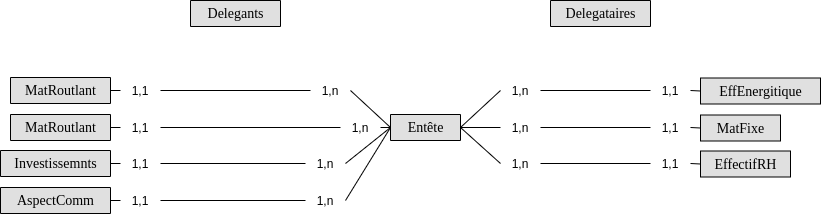
\includegraphics[scale=0.29]{images/MCD.png}}
%			\caption{Le modèle conceptuel des données}
%		\end{center}
%	\end{figure}
%	\subsubsection{MCD des données des référentiels}
%	\begin{figure}[H]
%		\begin{center}
%			\fbox{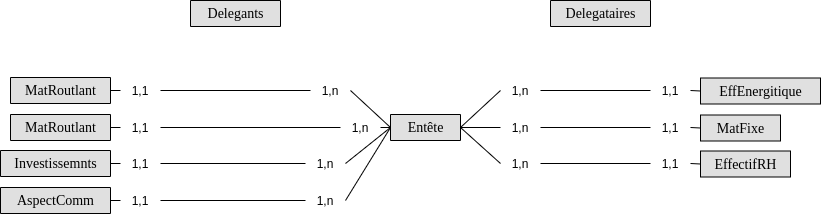
\includegraphics[scale=0.29]{images/MCD.png}}
%			\caption{Le modèle conceptuel des données}
%		\end{center}
%	\end{figure}
%	\subsubsection{MCD des données des avancements}
%	\begin{figure}[H]
%		\begin{center}
%			\fbox{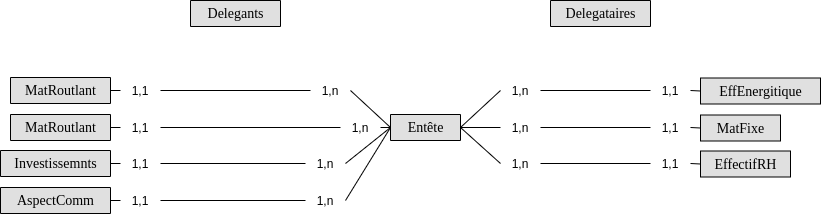
\includegraphics[scale=0.29]{images/MCD.png}}
%			\caption{Le modèle conceptuel des données}
%		\end{center}
%	\end{figure}
	\subsection{Le schéma relationnel de la base des données}
	Suite à ce qui précède, j'ai proposé le schéma relationnel de la base de données suivant:
%	\begin{figure}[H]
%		\begin{center}
%			\fbox{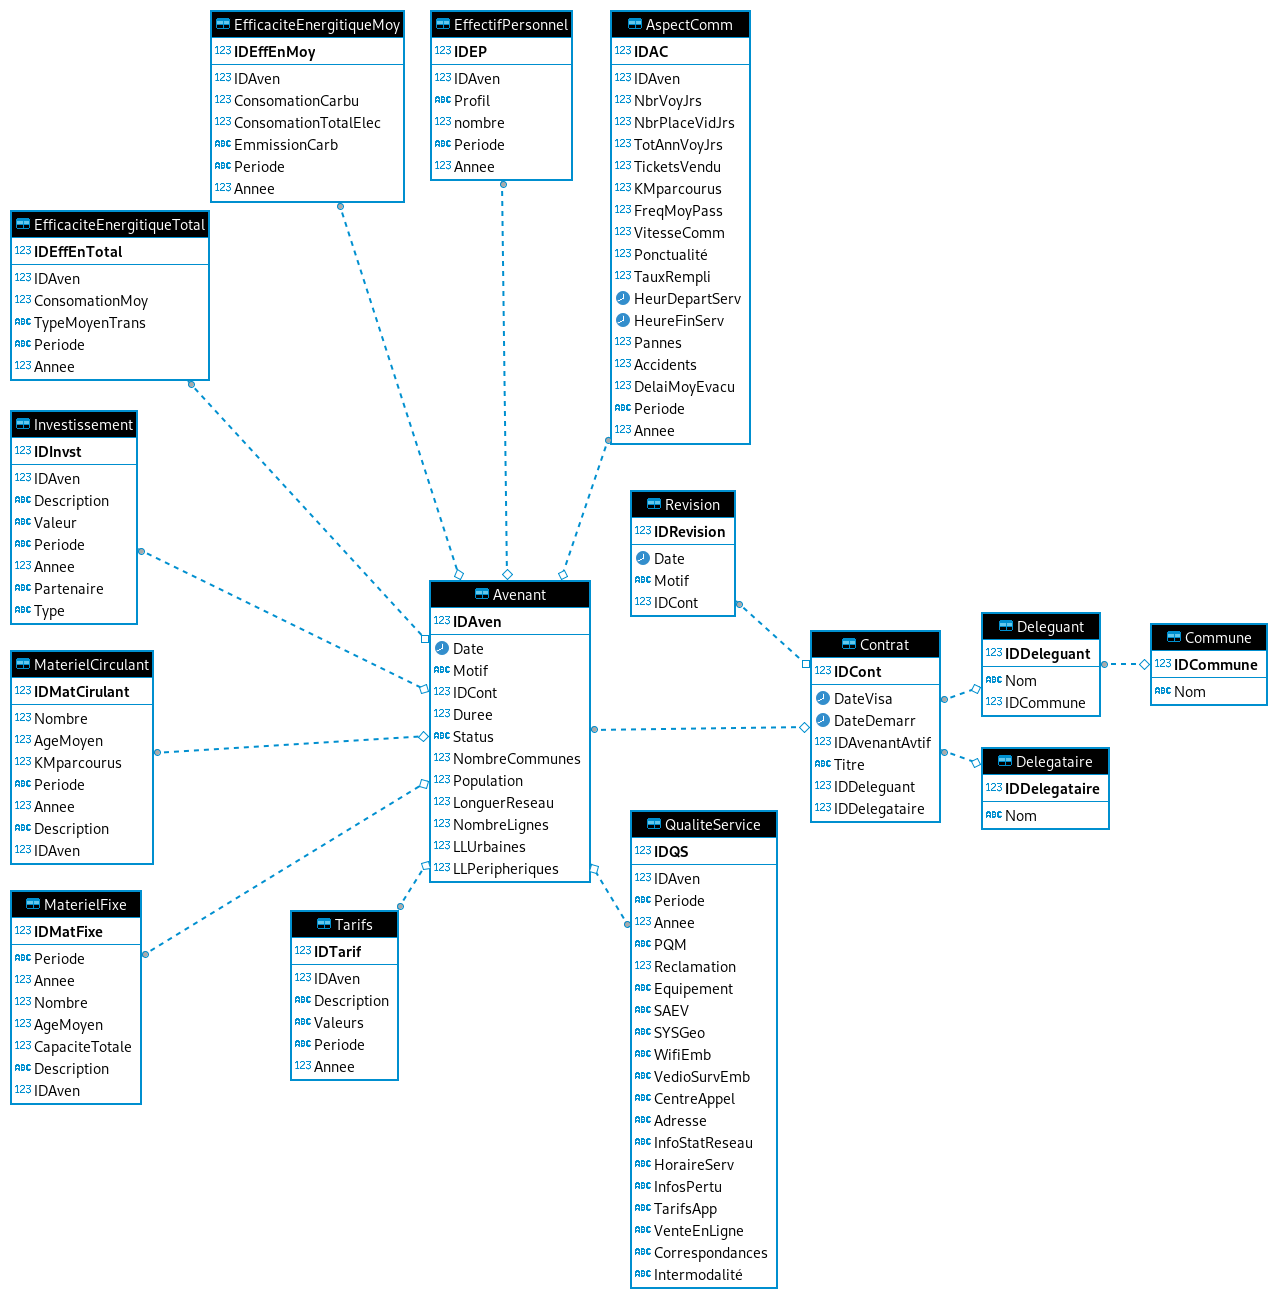
\includegraphics[scale=0.38]{images/database.png}}
%			\caption{Le modèle conceptuel des données}
%		\end{center}
%	\end{figure}
	\section{Étude structurale}
	\section{Étude comportementale}
	\section{Récapitulatif}
	\chapter{Réalisation et mise en œuvre}
	\fancyhead[R]{\textbf{Chapitre \thechapter: Réalisation et mise en œuvre}}
	\fancyhead[L]{\hspace*{5cm}}
\end{doublespace}

\newpage

\appendix
\pagenumbering{alph} \setcounter{page}{1}
\chapter{Références}

\begin{itemize}
	\item[•] %\textbf{Rapport en \LaTeX:} \url{https://github.com/abdorah/stage2021}
\end{itemize}

\chapter{Bibliographie}

\section{Cours}
\section{Sites Web}
\section{Documentations}

\end{document}
